\begin{savequote}[8cm]
\textit{Es müsse eine Art der Kerntheilung geben, durch welche die im Mutterkern enthaltenen Ahnenplasmen dergestalt auf die Tochterkerne vertheilt werden, dass jedem Tochterkern nur die halbe Zahl derselben zukomme.}

There must be a form of nuclear division in which the ancestral germ plasms contained in the nucleus are distributed to the daughter nuclei in such a way that each of them receives only half the number contained in the original nucleus.
  \qauthor{--- \cite{Weismann1887Ueber}}
\end{savequote}

\chapter{\label{ch:1-intro}Background}

\minitoc


\section{Aims}
Meiosis is a type of cell division in which the number of chromosomes is reduced by half to produce haploid gametes (sperm and egg cells)~\parencite{Ohkura2015Meiosis}. The primary aim of this research was to delineate the gene expression programme of spermatogenesis (during which meiosis occurs). Specifically, to identify which genes are expressed, in which cells, their degree of expression, and relative timing during spermatogenesis. With this atlas of expression data, we additionally aimed to infer the regulatory network controlling these expression patterns, as well as to predict protein function and in doing so identify targets for further characterisation. Finally, we aimed to carry out such characterisation for at least one of these targets.


\section{Motivations}

\subsection{Sexual Reproduction}
Reproduction is a fundamental property of all known life. Of the two empires of life Eukaryotes/Eukarya are able to reproduce sexually, and almost all do. The dominance of this trait has been estimated at roughly 99.9\% \parencite{White1978Modes}, with examples of exceptions being the Bdelloid rotifers - who lost the ability to reproduce sexually 60 Mya, and appear to be evolving by horizontal gene transfer \parencite{Debortoli2016Genetic}. This shared characteristic was likely present in the common ancestor of this empire and hence synapomorphic \parencite{Bernstein2013Evolutionary}. The sexual life cycle consists of an alternating halving of the genetic material/ploidy (by meiosis) to form haploid cells, followed by karyogamy (nuclear fusion). Meiosis (from Ancient Greek, meíōsis, “a lessening”) is a specialised form of cell division, in which genetic material is exchanged between the parental genomes (recombination). Recombination and independent assortment of homologous chromosomes generate genetic diversity and hence enable natural selection and evolution. Recombination also ensures balanced segregation at the reductional division which follows (no naturally occurring eukaryotes have a single chromosome - although synthetic yeast has been engineered - \cite{Shao2018Creating}).

The mechanisms of meiosis have important consequences for the evolution, fertility, and speciation of sexually reproducing organisms~\parencite{Davies2016Reengineering,Hassold2007Origin}. 


\subsection{Disease}
As the process of gamete generation, errors in meiosis can cause genetic disease in offspring. In some sense the most extreme version is complete infertility, affecting around 10\% of humans (with many being of unexplained cause) \parencite{Datta2016Prevalence, Hamada2011Unexplained}. Other errors can be compatible with fertilisation but not full gestation resulting in miscarriage (affecting around 13\% of pregnancies overall, but over 50\% for mothers over the age of 45 years - \cite{Magnus2019Role}). Others errors are compatible with birth but result in incurable disease such as some aneuploidies \parencite{Hassold2007Origin} and microdeletion syndromes caused by non-allelic homologous recombination \parencite{Myers2008common}.


A better understanding of the mechanisms of spermatogenesis and meiosis could aid in the prevention of such diseases. Additionally, determining the factors required for \emph{in vitro} spermatogenesis could enable the treatment of male infertility in addition to facilitating further research \parencite{Zhou2016Complete}.

While enabling the production of healthy offspring is one aim of reproductive medicine, \emph{preventing} fertilisation (usually but not always, temporarily) is also extremely important for the health of both mother and child \parencite{Cleland2012Contraception}. Hence the development of contraceptives is another key goal of reproductive science, and one for which a clearer delineation of testis specific genes could aid \parencite{Schultz2003multitude}.


\subsection{Curiosity}
As with many scientific endeavours curiosity is also a major driver of this research. The testis is a most unusual tissue especially at the transcriptional level. The testis has the highest number of tissue enriched genes out of the 32 tissues profiled in the Human Protein Atlas ($>$ five-fold higher mRNA levels in one particular tissue as compared to any other), with 1,057 enriched genes out of a total 2,489 across the 32 tissues~\parencite{Djureinovic2014human,Mele2015Human, Uhlen2015Tissuebased, Uhlen2016Transcriptomics, TheHumanProteinAtlas2019human}. This is over twice as many as the second highest tissue the cerebral cortex which is perhaps considered the most complex tissue functionally, and with which the testis shares a surprising similarity \parencite{Guo2005Transcriptomic, Djureinovic2014human, Uhlen2015Tissuebased}. More recent studies using single-cell sequencing have underscored the distinct transcriptional state of the testis (\cite{Han2018Mapping} and figure \ref{fig:MCA_PCA}). The testis is also one of a few immune privileged sites in the human body \parencite{Fijak2006testis}.


\begin{figure}[H]
	\centering
	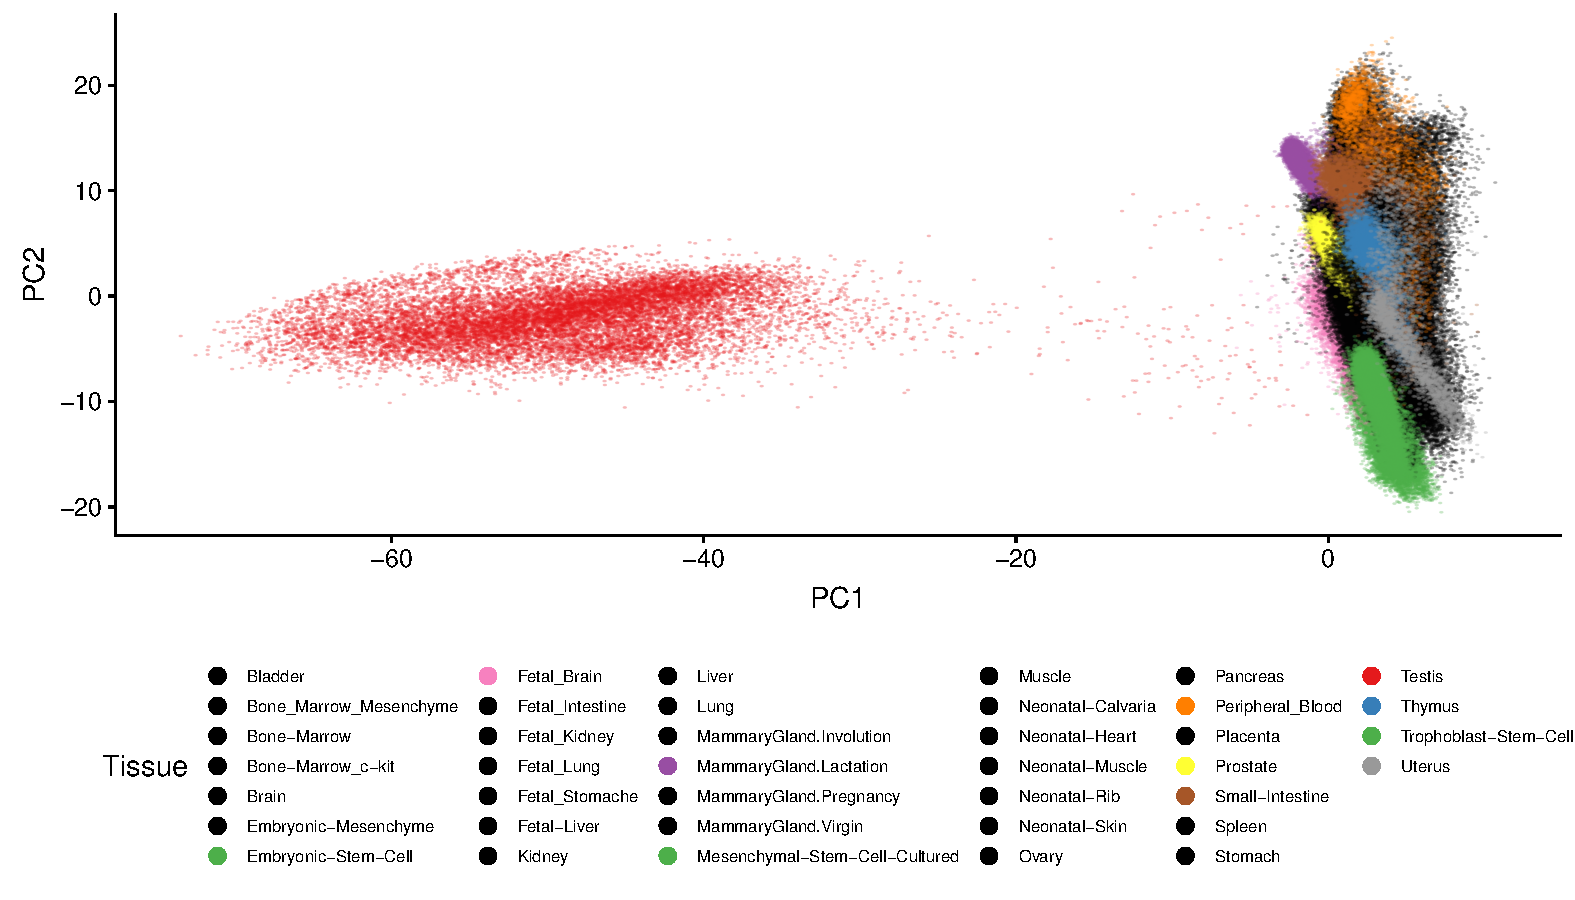
\includegraphics[width=\textwidth]{figures/intro/MCA_PCA.pdf}
	\caption[Testis PCA (MCA)]{PCA of single cell RNAseq of 50 different tissues and cell types from over 400,000 cells from the mouse. Data from~\cite{Han2018Mapping}}
	\label{fig:MCA_PCA}
\end{figure}


 The previous two properties have lead to the use of testis expressed genes as targets for cancer immunotherapy (cancer testis antigens) as when re-expressed in cancers they provide a distinguishing biomarker \parencite{Whitehurst2014Cause}.

Chromatin undergoes massive remodelling during spermatogenesis ultimately resulting in most (90/99\% in human/mouse) of the histones being replaced by crosslinked protamines, leading to the cessation of transcription \parencite{Rathke2014Chromatin}. This necessitates long term mRNA storage ($>$5 days) before translation \parencite{Kleene2013Connecting}.

Sperm are a highly specialised cell, despite being a single cell and unable to transcribe new mRNA they must perform many of the functions of the whole organism including motility, sensing the environment (chemotaxis), and defence from attack (from the female immune system) \parencite{Kaupp2008Mechanisms, Thompson1992Leukocytic}. Indeed they are able to survive and even fertilise after more than three days in the female reproductive tract \parencite{Gould1984Assessment,Wilcox1995Timing}.

Meiosis itself of course is also unique, with paternal and maternal homologous chromosomes being blissfully unaware of each other in somatic cells, until pairing in meiosis in the germline.

%Incomplete cytokinesis


\subsection{Mapping Projects of Science}
Much of science can be characterised as the creation of maps. The discovery, description and cataloguing of various types of elements, which is often dismissed as `merely descriptive', is a fundamental bedrock of many sciences \parencite{Grimaldi2007Why}. Maps are often useful in two senses, they serve as a reference of what's already known, but they also arrange current knowledge in such a way as to provide a prediction of the unknown. For example Mendeleev's periodic table both catalogued the known elements but left gaps for new discoveries. Equally with the Standard Model in physics. Darwin and others made extensive catalogues of past and present diversity of life, eventually resulting in the concept of evolution by natural selection. Cataloguing the ratios of offspring phenotypes lead to Mendel's laws.

Our maps of protein function are woefully incomplete, with more than 3,000 (15\%) of human genes not even having a biological process annotation (and a similar \% in the more experimentally amenable organisms \textit{S. cerevisiae} and \textit{S. pombe}) \parencite{Wood2019Hidden}. Even genes with at least one annotation or paper are often incompletely or even incorrectly characterised. Significant bias exists against initiating research into a gene of unknown function \parencite{Edwards2011Too, Stoeger2018Largescale, Haynes2018Gene}. This can be partially attributed to risk averse incentives in scientific funding and evaluation. In addition, for many proteins of unknown function there are limited tools available such as antibodies, making even simple characterisation difficult (for example immunofluorescence or immuno-precipitation based assays).


\subsection{Maps of Protein Function}
Genome sequencing projects have provided a single base resolution maps of many organisms genomes (thousands of eukaryotes - \cite{Genome}). This relatively unbiased approach has uncovered many genes of unknown function and has accelerated their characterisation. For example, by enabling the inference of molecular function from homology with known domains, and by facilitating sequence based detection and cloning. Ultimately much of what we care about is at the level of a phenotype such as infertility, and GWA studies provide one way to potentially associate genes with such phenotypes \parencite{Gajbhiye2018Complex}. However, \emph{if} a causal gene can be confidently identified for an associated SNP, because the phenotypes are usually broad, this often tells us nothing about the molecular function of a gene which then requires substantial follow up research which is frequently not undertaken \parencite{Visscher201710, Gallagher2018PostGWAS, Struck2018impact}.

In a reverse genetics approach specific mutations are created and the phenotypic results are investigated. The International Mouse Phenotyping Consortium aims to generate and broadly phenotype knockout mice for every protein coding gene, with a current catalogue of over 5,000 null mice models \parencite{2004Knockout,Meehan2017Disease, Birling2019resource}.

Other atlases such as the Human Protein Atlas and GTEx instead start from the first step in a gene's function, providing transcriptomic data enabling association of co-expressed genes and association of tissue specific genes with the function of those tissues. However, bulk tissues are too heterogeneous and large scale to provide much useful insight into molecular function. Through a similar argument, proteins with co-varying abundances and protein-protein interactions can also implicate functions.

A protein's structure is often more conserved than its sequence and can give direct mechanistic insight into its function \parencite{Illergard2009Structure, Sousounis2012Conservation}. Despite being less able to take advantage of advances in high throughput next generation sequencing technology, over 144,000 structures are held by the Protein Data Bank, many deposited by structural genomics programs, but still many protein families lack a single structure \parencite{wwPDBconsortium2019Protein, Grabowski2016Impact, Khafizov2014Trends}.

Recently, droplet based single cell RNAseq technologies have enabled higher resolution high-throughput characterisation of gene co-transcription. A number of mapping projects have been launched including the Human Cell Atlas and Mouse Cell Atlas as well as other tissue specific maps including the one we present here, helping to provide much higher resolution clues for the function of unstudied genes \parencite{Regev2017Human,Regev2018Human,Han2018Mapping,TheTabulaMurisConsortium2018Singlecell}.


%%%%%%%%%%%%%%%%%%%%%%%%%%%%%%%%%%%%%%%%%%%%%%%%%%%%%%%%%%%%%%%%%%%%%%%%
\section{Measuring Gene Expression}
%%%%%%%%%%%%%%%%%%%%%%%%%%%%%%%%%%%%%%%%%%%%%%%%%%%%%%%%%%%%%%%%%%%%%%%%

Expression is the process in which information contained within the genome manifests as a phenotype. This involves generation a functional biomolecule such as proteins but sometimes RNA (most importantly the ribosome). The first step in expression is the generation of messenger(m) RNA and there are a number of different technologies available to quantify the amount of mRNA - each providing different types and amounts of information.

Physical limits make it challenging to sensitively and accurately quantify gene expression. mRNA is <5\% of total RNA in a cell, with the rest comprising of ribosomal and transfer RNA \parencite{Warner1999economics}. Total RNA content per eukaryotic cell is approximately 20pg, with <1pg of mRNA, corresponding to roughly <500,000 mRNA molecules \parencite{Roozemond1976Ultramicrochemical, Uemura1980Agerelated, Tang2011Development}. Most genes have mRNA copy numbers of 1-100 per cell, up to a maximum of perhaps 1,000 \parencite{Marguerat2012Quantitative, Macaulay2014Single}. At the level of individual cells, mRNA synthesis is ``bursty'' introducing further biological heterogeneity in expression measurements \parencite{Raj2006Stochastic, Chubb2006Transcriptional}.

\subsection{In Situ Hybridization}
In Situ Hybridisation, first described by \cite{Gall1969Formation}, uses a probe (either RNA or DNA) which is incubated with fixed cells and binds to a target mRNA by complementary binding and can then be visualised. This has the advantage of being single cell resolution, and even allowing subcellular localisation to be observed.

Visualisation of the probe initially used radioactive labelling which was low resolution, expensive, unstable, and dangerous. However, this was overcome by using biotinylated probes couples with secondary detection \parencite{Singer1982Actin} and later directly fluorescent probes (FISH) \parencite{Kislauskis1993Isoformspecific}.

This sensitivity of this technique has been further increased by using multiple probes per target RNA, enabling the detection of individual mRNA molecules (single molecule smFISH - \cite{Femino1998Visualization, Raj2008Imaging}. In addition, multiplexed detection schemes using multiple cycles of sequential hybridization and imaging such as SeqFISH(+) \parencite{Lubeck2014Singlecell,Eng2017Profiling,Eng2019Transcriptomescale} and MERFISH \parencite{Chen2015Spatially, Moffitt2016Highthroughput, Moffitt2016Highperformance, Xia2019Multiplexed} are able to measure many (up to 10,000) RNA targets. These methods have the advantage that amplification is not necessarily required and the high sensitivity allows single molecules to be detected. Furthermore, by measuring nuclear vs cytoplasmic localisation or by using probes to introns, mRNA dynamics (``RNA velocity'') and isoform usage can also be measured \parencite{Shah2018Dynamics, Xia2019Spatial}.

%(barcodes??)

\subsection{RT-qPCR}
Reverse transcription quantitative real-time PCR measures PCR products during the amplification by using fluorescent detectors \parencite{Gibson1996novel, Heid1996Real, Chiang1996Use}. This technique is able to detect a single mRNA molecule, and has become the gold standard in expression quantification. However, primers must be designed for each gene and any spatial information is lost \parencite{Palmer2003New, Wong2005Realtime}.

Furthermore, due to the exponential amplification, small differences in reverse transcription, primer efficiency, or initial starting amounts and contamination can lead to inaccurate quantification. Therefore, efficiency and validated reference genes must be established by separate experiments \parencite{Bustin2009MIQE}.

\subsection{Northern Blot}
The Northern blot  is one of the earliest methods for measuring mRNA levels \parencite{Alwine1977Method}. It consists of RNA extraction, separation by gel electrophoresis, followed by transfer by blotting onto a membrane and finally detection by complementary hybridisation with a radioactive/fluorescent probe. Northern blotting still remains a useful technique when information about the relative sizes of transcripts is required.

\subsection{Microarrays}
A microarray is typically a glass slide coated with cDNA oligomers. mRNA with polyA tails can be extracted from total RNA using oligo(dT) beads, reverse transcribed to cDNA, fluorescently labelled, and washed over the array \parencite{Schena1995Quantitative, DeRisi1996Use, Schulze2001Navigating}. The fluorescent intensity is a measure to the abundance of mRNA in the sample. This approach allowed whole transcriptome quantification and was wildly popular, with the EBI ArrayExpress database passing 100,000 hybridisations in 2008 \parencite{Rustici2008Data}.

\subsection{Bulk RNA Sequencing}
No sooner however, the reducing cost of DNA sequencing among other things led to the use of this technology to quantify the transcriptome \parencite{Mortazavi2008Mapping, Cloonan2008Stem, Wilhelm2008Dynamic, Lister2008Highly, Nagalakshmi2008Transcriptional}. mRNA is extracted as for microarrays, fragmented, and sequenced using short read NGS technology before being re-mapped to the genome. This has the advantage over microarrays that the sequence of hybridisation probes does not need to be designed from an already known transcriptome reference. Enabling, for example, novel transcripts and splice isoforms to be discovered. RNAseq provides a digital read out in comparison to the analogue signal from microarrays which limited its replicability across platforms. In addition, the dynamic range is much greater than for microarrays in which the signal saturates when all probes are bound and at low concentrations non-binding is favoured \parencite{Zhao2014Comparison}. RNAseq also enables detection of sequence variants and allele specific expression. For these reasons RNAseq has become the standard method for profiling the transcriptome \parencite{Stark2019RNA}.

As it's based on standard sequencing technology RNAseq benefits from advances in next generation sequencing. For example, long read technology from PacBio enables full transcript (cDNA) sequencing - enabling the unambiguous identification of transcript isoforms which has to be inferred using the fragmentation approach of short read sequencing \parencite{Sharon2013singlemolecule, Cartolano2016cDNA}.
Oxford Nanopore sequencing infers the sequence of polynucleotides from the change in current as they pass through a nanopore embedded within a membrane across a voltage. In addition to being able to sequence long reads like PacBio \parencite{Oikonomopoulos2016Benchmarking}, this technology is also able to sequence mRNA directly, bypassing the fragmentation, reverse transcription, PCR amplification and size selection steps, reducing opportunities for bias \parencite{Garalde2018Highly, Workman2019Nanopore}. Furthermore Oxford Nanopore sequencing is able to quantify polyA lengths and detect RNA modifications such as N6-methyladenine.

\subsection{Single Cell RNA Sequencing}
RNA sequencing of single cells (scRNAseq) was first performed by \cite{Tang2009mRNASeq} using a modified amplification protocol previously used in single cell microarray studies, generating a dataset of five cells. By incorporating a cell-unique barcode during reverse transcription, cells can be multiplexed (pooled post mRNA capture and separated in silico) reducing cost and increasing the cell throughput to \textasciitilde100 \parencite{Islam2012Highly}. Using automated liquid handling robots and 384 well plates enabled the generation of a 4,468 cell dataset \parencite{Jaitin2014Massively}. Such scale is also possible using subnanolitre well arrays \parencite{Bose2015Scalable, Fan2015Combinatorial, Gierahn2017SeqWell}. The use of oil immersed nano-droplets to encapsulate individual cells with lysis buffer and polyT coated beads further increased throughput up to 44,808 cells \parencite{Macosko2015Highly, Klein2015Droplet}. Both microwell and nanodroplet isolation methods have now been used to generate datasets at an additional magnitude of scale with 400k, and 690k cells respectively \parencite{Saunders2018Molecular, Han2018Mapping}. This exponential scaling of single cell RNAseq datasets appears to be continuing with one dataset including more than 2 million cells \parencite{Cao2019singlecell} and creation of datasets with tens of thousands of cells being common especially using the commercial Chromium platform from 10X genomics (figure \ref{fig:scStudies}, \cite{Zheng2017Massively, Svensson2018Exponential}).

\begin{figure}[H]
	\centering
	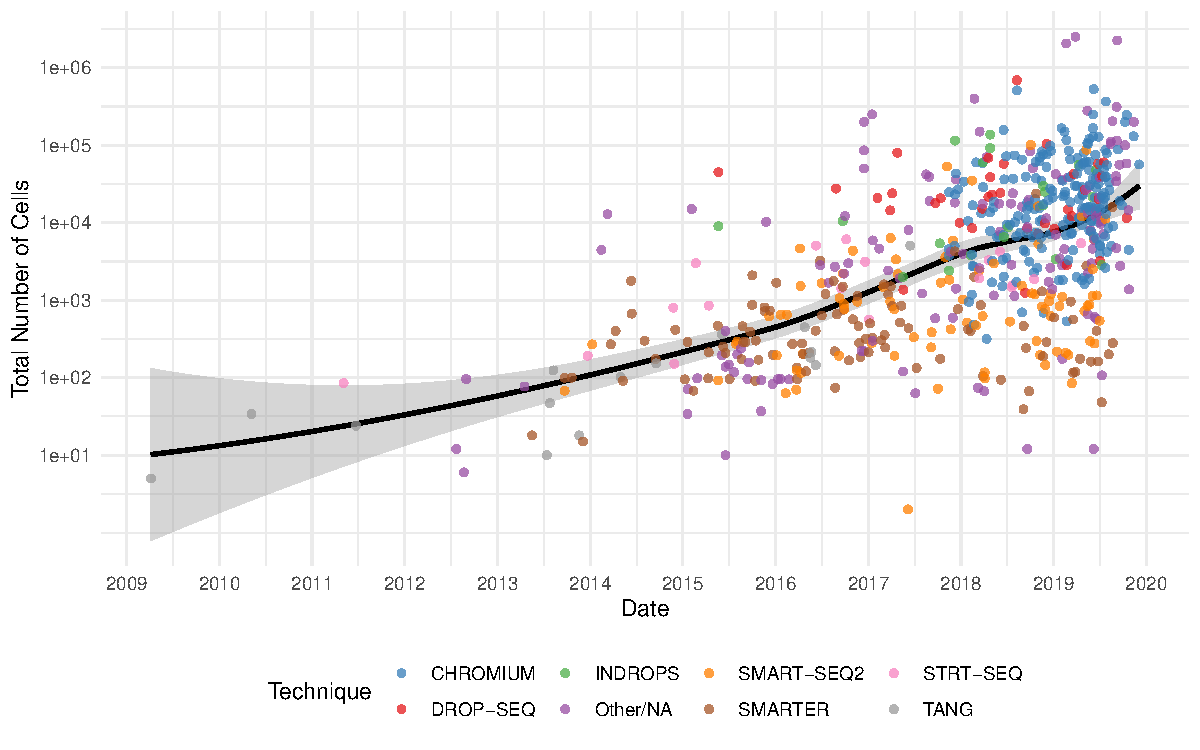
\includegraphics[width=\textwidth]{figures/intro/scStudies.pdf}
	\caption[scRNAseq Publications]{Exponential scaling of Single Cell RNAseq studies. Data from~\cite{Svensson2019curated}}
	\label{fig:scStudies}
\end{figure}

In scRNAseq, due to the low amount of starting material, many rounds of PCR amplification are required to generate sufficient material for sequencing. However this amplification step introduces significant bias, skewing the resulting levels \parencite{Best2015Computational}. To alleviate this unique barcodes named UMIs (unique molecular identifier) can be included in each poly-dT probe, in addition to the unique barcode for each cell (1 per bead) \parencite{Kivioja2012Counting,Islam2014Quantitative}. This enables each original mRNA molecule to be counted as a single molecule, in effect providing an absolute count of molecules rather than relative abundance as in standard bulk RNAseq. However, UMIs do not alleviate bias due to preferential sampling of molecules by RT or PCR primers \parencite{Kou2016Benefits}. In addition, as the UMI and cellular barcode is on the 3' end of the transcript, after fragmentation only the fragments at the 3' end will be sequenced. This bias is in addition to the 3' bias from polyA selection \parencite{Wan2012Modeling, Lahens2014IVTseq}. This 3' bias precludes analysis of transcript isoforms as only the 3' end of the fragment is sequenced (as most transcripts sharing the 3' UTR, and the 5' read contains only the UMI and cell barcode). However, some isoform information is available due to the use of alternative 3' UTRs (and possibly by internal polyA priming), if pseudo-alignment is used to generate transcript compatibility counts \parencite{Nam2002Oligo, Ntranos2019discriminative}.

Despite what the name suggests, some cells will actually be multiple cells, due to two (or more) cells being captured into the same droplet or well, named ``doublets''. The doublet rate is determined by concentration of cells in the solution / flow rate into the droplets. By Poisson sampling a flow rate can be calculated to minimise doublets but also balance the cost of empty beads. The doublet rate can be determined experimentally by mixing single cells from two different species, in which case double species encapsulations can be detected by the different gene sequences (and the total number of doublets calculated as double that) \parencite{Macosko2015Highly}.  Doublets can also be detected by natural genetic variation when multiplexing multiple genetically distinct individuals of the same species \parencite{Kang2018Multiplexed}. Artificial genetic variation can also be added by using oligonucleotide-tagged antibodies \parencite{Stoeckius2018Cell}. Recently a method using whole-transcriptome pre-indexing was proposed, enabling overloading of droplets and a corresponding massive increase in throughput \parencite{Datlinger2019Ultrahigh}. A number of computational tools have also been created to attempt identification of doublets by simulating artificial doublets \parencite{Wolock2019Scrublet, McGinnis2019DoubletFinder}. Another way in which mRNA can cross contaminate across cells is if damaged cells leak mRNA into the solution which is then captured.



\subsection{Spatial Sequencing}
A disadvantage in most single cell RNAseq methods is the loss of spatial information during cell dissociation and isolation. New methods have been developed to combine the spatial advantages of In Situ Hybridisation and the transcriptome wide nature of scRNAseq. One type of method ``in situ sequencing'' typically uses rolling circle amplification of an mRNA target resulting in a DNA nano-ball which is sequenced by ligation, achieving a resolution of 0.5-1$\mu$m for up to 1,000 genes \parencite{Lee2014Highly, Wang2018Threedimensional, Qian2018spatial}. Another approach ``spatial transcriptomics'' uses a spatially barcoded bead array which captures mRNA from an overlaid tissue, enabling quantification of all genes but with lower spatial resolution (2-100$\mu$m) than in situ sequencing \parencite{Stahl2016Visualization, Rodriques2019Slideseq, Vickovic2019Highdefinition}


\subsection{Nascent RNA Sequencing}
Although we say the previous methods measure ``expression'' we are actually measuring the total mRNA, which is the cumulative result of transcription minus mRNA degradation. Methods such as GRO/PRO/NET-seq allow profiling of nascent mRNA, revealing which genes are being transcribed at a specific time-point \parencite{Core2008Nascent, Churchman2011Nascent, Mahat2016Basepairresolution}.


\subsection{Proteomics}
Given that we (mostly) ultimately care about \emph{protein} function, using mRNA as a proxy for this deserves some caveats and justification. Quantification of the full proteome, either by mass-spectrometry approaches or by nanopore protein sequencing, hold promise (with proteins being present in higher copy number than mRNA) but has yet to be fully realised \parencite[Reviewed in][]{Specht2018Transformative,Marx2019dream}. Whilst there are many factors resulting in a decoupling of mRNA and protein levels, protein levels are largely determined by mRNA concentrations \parencite[Reviewed in][]{Liu2016Dependency}.




%%%%%%%%%%%%%%%%%%%%%%%%%%%%%%%%%%
%%%%%%%%%%%%%%%%%%%%%%%%%%%%%%%%%%
%%%%%%%%%%%%%%%%%%%%%%%%%%%%%%%%%%


\section{Gametogenesis}
Gametogenesis is the process by which primordial germ cells develop into either spermatozoa in the male (spermatogenesis) or ovum in the female (oogenesis). Whilst equally important to spermatogenesis, oogenesis is studied far less (1,099 vs 359 articles indexed in PubMed 2018). This is likely partially due to difficulties in studying oogenesis compared to spermatogenesis. In oogenesis prophase I up to diplotene occurs in the ovary of the fetus before birth at which point meiosis is arrested (``Dictyate''), making experiments more challenging.

\subsection{Testis Anatomy}
Whilst the fundamental features of spermatogenesis and oogenesis are the same, spermatogenesis is organised into a specific structure. The testis is composed of seminiferous tubules surrounded by somatic accessory cells such as Leydig cells which produce testosterone. Germ cells are located within the tubule supported by a somatic cell type named Sertoli cells. The germ stem cells are located at the basal surface next to the tubule wall, and more differentiated germ cells are located progressively inwards towards the lumen/apical surface of the tubule (figure~\ref{fig:histology}).

\begin{figure}[H]
	\centering
	\includegraphics[width=\textwidth]{figures/intro/histology.png}
	\caption[Testis Anatomy]{Cross section of a seminiferous tubule in testis with the main cell types labelled, reproduced from~\cite{Junqueira2005Basic}}
	\label{fig:histology}
\end{figure}

Within a given region of tubule, entry into spermatogenesis is coordinated such that each developing germ cell belongs to a cohort of the same stage. The rate of entry is precisely timed (every 8.6 days in mice) and shorter than the total developmental time (35 days in mice, >70 in humans) such that in any given tubule section different generations of germ cells occur in layers of particular cell type combinations (figure \ref{fig:cycle}, \cite{Oakberg1956Duration,Clermont1969Duration, Heller1969Human}). This is called the cycle of the seminiferous epithelium and it's possible to stage each combination of cells using periodic acid‐fuchsin sulfurous acid staining (14 combinations in rat, and 12 in mouse) \parencite{Leblond1952Spermiogenesis, Leblond1952Definition, Oakberg1956description}. The cycle starts at a different time laterally along the tubule (in a so called ``wave''), ensuring continuous production of sperm, although the very first wave is synchronous - a property sometimes used to purify or enrich for specific stages.

\begin{figure}[H]
	\centering
	\includegraphics[width=\textwidth]{figures/intro/cycle.png}
	\caption[Seminiferous Cycle]{Association of different germ cells during the seminiferous epithelial cycle~\cite[Reproduced from ][]{Monesi1978Chapter}}
	\label{fig:cycle}
\end{figure}


\subsection{Spermatocytogenesis}
Prior to meiosis there are a number of \emph{mitotic} divisions, amplifying the true spermatogonial stem cell \parencite{Oakberg1971Spermatogonial, Huckins1971spermatogonial}. The first set of these divisions occur asynchronously between stage stages X and II \parencite{Rooij2001Proliferation}. There are up to four or five divisions in this first proliferation and the resulting cells are named $A_{single}$, $A_{paired}$, $A_{aligned-4}$ $A_{aligned-8}$, $A_{aligned-16}$. At stage VIII all the $A_{aligned}$ cells differentiate (without division) into $A_1$ cells which are considered committed to the meiotic program and now divide in synchrony with the stages of the seminiferous cycle \parencite{Rooij2000All}. This commitment step is induced by a pulse of retinoic acid (Vitamin A metabolite), which induces expression of the Stra8 transcription factor in these cells (and pre-leptotene cells which occur in the same stage) \parencite{Griswold2012Initiating, Lin2008Germ, Zhou2008Expression, Hogarth2015Processive, Griswold2015Spermatogenesis}. A Vitamin A deficient diet results in lack of progression to $A_1$ spermatogonia, enabling an additional method to generate synchronised cells \parencite{Thompson1964Vitamin}. $A_1$ cells divide by mitosis into $A_2$, then $A_3$, and $A_4$ all of which are indistinguishable morphologically but occur at different stages of the seminiferous cycle \parencite{Rooij2000All}. $A_4$ cell divide into ``In'' cells (with intermediate levels of heterochromatin) and then into spermatogonial B cells before a final mitosis generates pre-leptotene spermatocytes \parencite{Rooij2000All}.

Meiosis is preceded by DNA replication much like in mitosis and so initiates from cells that are 2n, 4c (n = ploidy / number of centromeres; c = number of chromosomes).

\subsection{Prophase I of Meiosis I}
During meiosis there is an extended prophase I (lasting 14 days in mice), which is itself divided into a number of stages: Leptotene (thin ribbon), Zygotene (union ribbon), Pachytene (thick ribbon), and Diplotene (double ribbon) - originally defined by the morphology of the chromosomes through a light microscope (sometimes suffixed -nema using the greek for ``thread'' instead of ``ribbon'') \parencite{DeWiniwarter1900Recherches, Gregoire1907formation, Wilson1912Studies, Zickler1998leptotenezygotene}.

However, with the discovery of the synaptonemal complex (figure \ref{fig:synaptonemal_complex}, a proteinaceous scaffold that forms along the chromosomes, \cite{Moses1956Chromosomal, Fawcett1956FINE}), the stages are also now defined by the configuration of this structure \parencite{Zickler2015Recombination}. Lepotene being the stage in which the lateral elements form along the axis of homologous chromosomes, Zygotene starts at the formation of the first transverse filaments and the central element between the homologous chromosomes \parencite{Moens1968structure}, Pachytene is defined as the stage in which all chromosomes (excepting the sex) are fully synapsed, and Diplotene when the synaptonemal complex starts to disassemble \parencite{Moses1958Relation, Moses1977Synaptonemal}. The lateral elements are formed of SYCP2 \& SYCP3 proteins, whereas the central element is formed of SYCE1, SYCE2, SYCE3, SIX6OS1, and TEX12, with SYCP1 forming the transverse elements connecting the two \parencite[reviewed in][]{Zickler2015Recombination, Gao2018Zipping, Kaniecki2018change, Dunce2018Structural}. The formation of the axis is dependent on a meiosis specific cohesin complex (comprised of REC8, RAD21L, SMC1B, STAG3) which encircles the sister chromatids \parencite[reviewed in][]{Rankin2015Complex, Ishiguro2019cohesin}.

\begin{figure}[H]
	\centering
	\includegraphics[width=\textwidth]{figures/intro/synaptonemal_complex.pdf}
	\caption[Synaptonemal Complex]{Schematic of the synaptonemal complex at different stages during Prophase I~\parencite[Reproduced from ][ CC BY 0 Licence]{Gaysinskaya2018MOESM1, Gaysinskaya2018Transient}}
	\label{fig:synaptonemal_complex}
\end{figure}

In Leptotene SPO11, a conserved topoisomerase like protein, acts with mTopVIB (GM960 in mice) to create \textasciitilde300 programmed double-strand breaks (DSBs) \parencite{Sun1989Doublestrand, Keeney1997MeiosisSpecific, Bergerat1997atypical, Cole2012Homeostatic, Vrielynck2016DNA, Robert2016TopoVIBLike, Li2019highresolution}. In species able to pair homologues without recombination (\textit{Drosophila melanogaster} and \textit{Caenorhabditis elegans}) only ~20-30 breaks are formed, while in other species such as lilly over 2,000 DSBs are formed (as assessed by RAD51 foci counts) \parencite{Terasawa1995Localization}. Like other topoisomerases the two SPO11 molecules form covalent bonds with each end of the DNA \parencite{Neale2005Endonucleolytic}.

The activity of SPO11 depends on pre-DSB recombinosomes containing MEI4, REC114, IHO1 (aka CCDC36, MER2) and ANKRD31 which are bound to unsynapsed axes via HORMAD1/2 \parencite{Kumar2010Functional,Panizza2011Spo11Accessory, Stanzione2016Meiotic, Kumar2018Mouse, Papanikos2019Mouse, Boekhout2019REC114}. MEI1 is also required for DSBs, and WDR61 is hypothesised to be required as it's a homologue of Ski8/Rec14 which is required in \textit{S. cerevisiae} \parencite[reviewed in][]{Kumar2010Initiation, Lam2015Mechanism}. pre-DSB recombinosome recruitment also depends on meiotic cohesin \parencite{Bhattacharyya2019Prdm9}.

The DSB lesions are initially processed in much the same way as DSBs in mitotic cells: they are rapidly recognised by CtIP-(SAE2)-activated MRN complex (MRE11, RAD50, NBS1), which possesses 3'-5' nuclease activity. They are then further resected by either the 5'-3' exonuclease EXO1, or DNA2 nuclease with the BTRR complex (BLM (SGS1) helicase, TOP3A, RMI1, RMI2 \parencite{Daley2014Multifaceted}) resulting in the release of SPO11 bound oligos (figure \ref{fig:molecular_recombination}, \cite[Reviewed in][]{Symington2014End, Schiller2014Structural, Lam2015Mechanism}). MRN recruits the ATM kinase which in turn activates a cascade of DNA damage response activities including phosphorylation of the histone variant H2AX \parencite{Marechal2013DNA}. RPA then coats the single stranded DNA, but is replaced by RAD51 and the meiosis specific protein DMC1, with the aid of BRCA2 \parencite{Liu2010Human, Jensen2010Purified, Shi2019Dual}. MEIOB and SPATA22 are RPA homologues that are also recruited to DSBs, but their function is unknown \parencite{Xu2017Meiosisspecific}.


\begin{figure}[H]
	\centering
	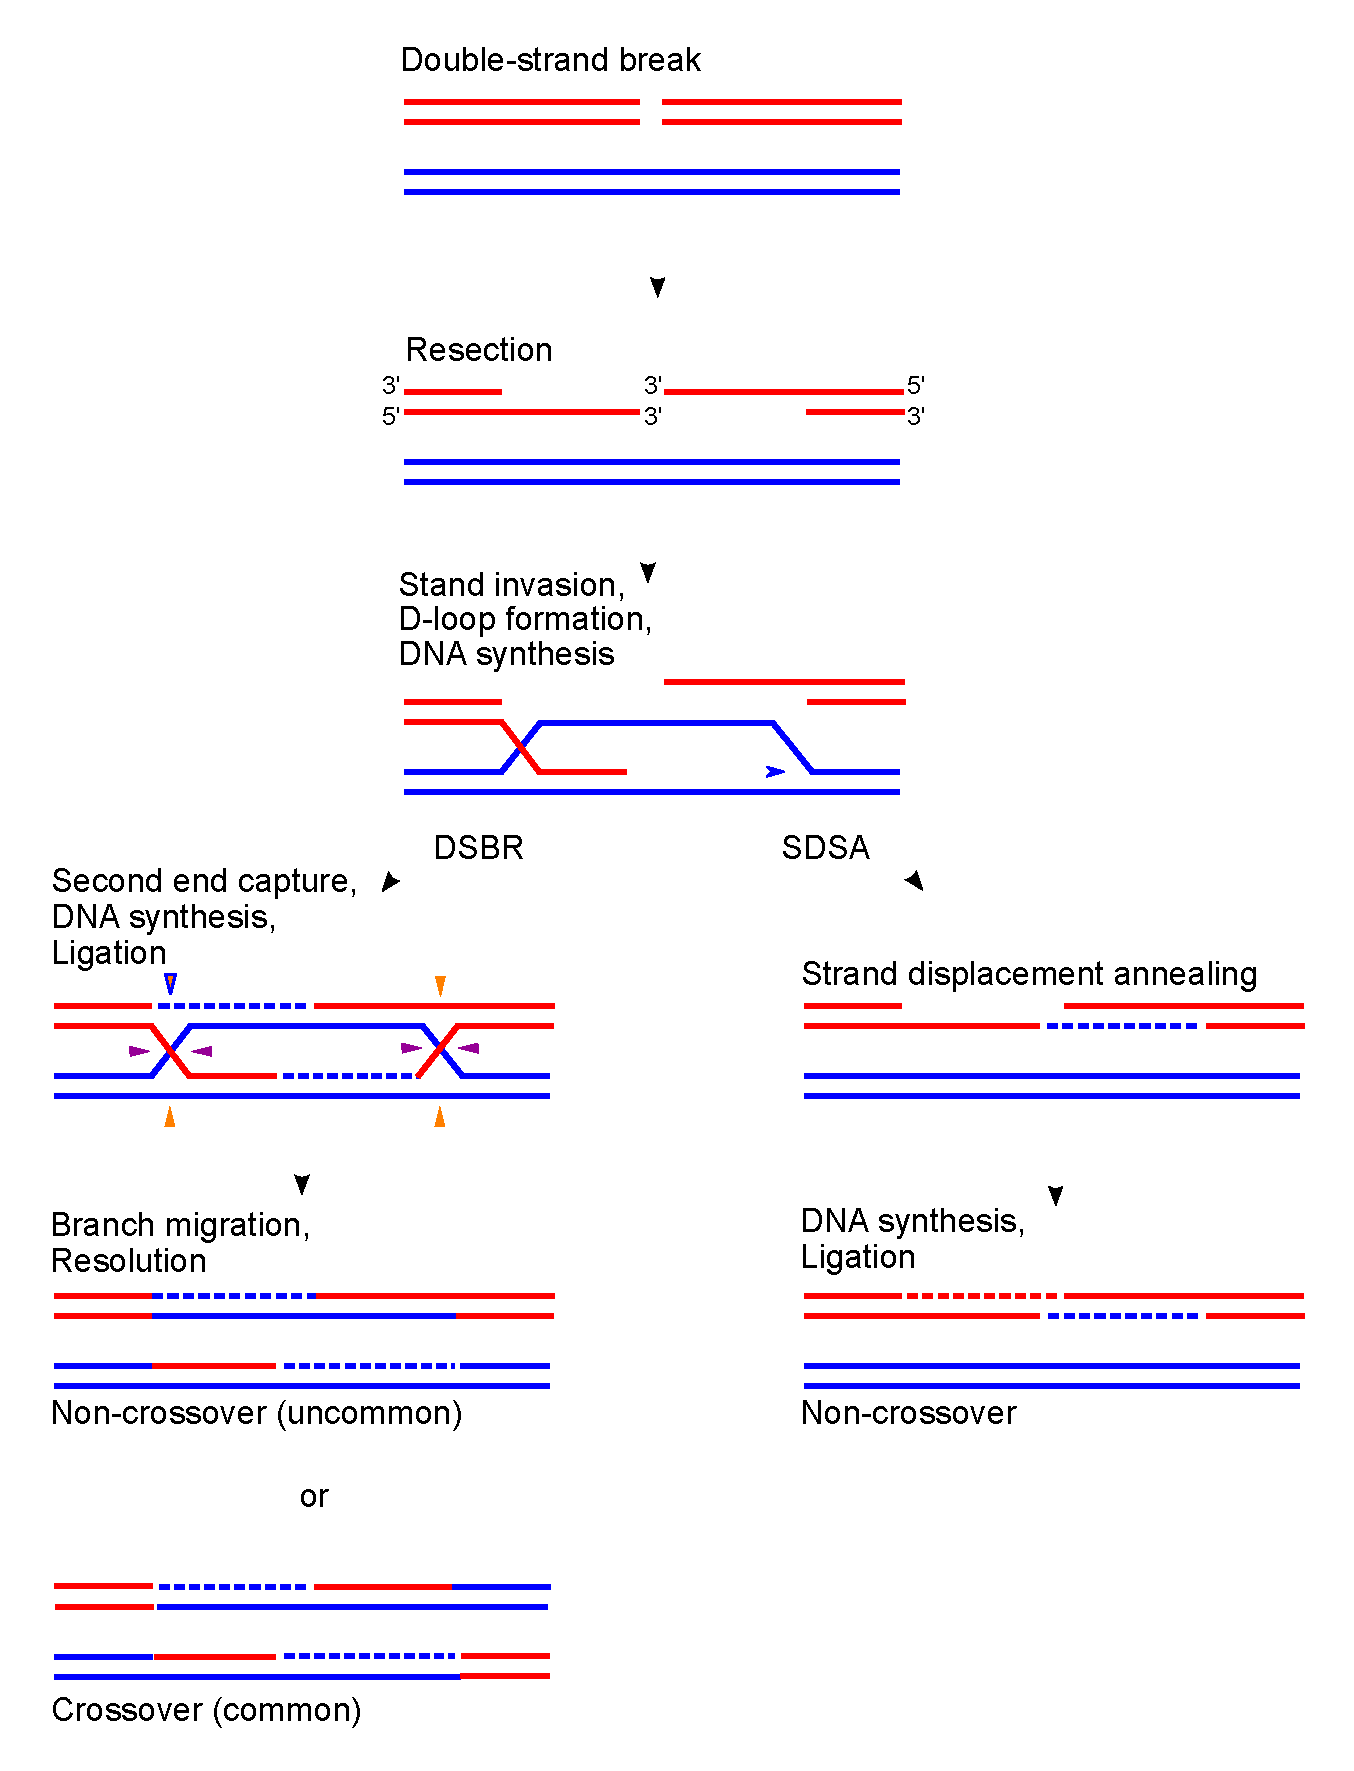
\includegraphics[width=\textwidth]{figures/intro/recombination.jpg}
	\caption[Molecular Recombination]{Schematic of the recombination process and associated proteins}
	\label{fig:molecular_recombination}
\end{figure}

RAD51 and DMC1, along with other helper proteins, form a right handed bipolar helical filament (where DMC1 is oriented at the broken end, with 3bp per monomer), able to invade the homologous chromosome to search for a homologous template for repair \parencite{Sehorn2004Human, Cloud2012Rad51, Brown2015Small, Brown2015DNA, Crickard2018Spontaneous}. This filament is brought / binds to duplex DNA (perhaps helped by RAD51AP1, PALB2, or HOP2-MND1, \cite{Petukhova2005Hop2}) and probes for homology using base-flipping \parencite{Gupta1999Rapid, Folta-Stogniew2004Exchange}. This search likely involves a combination of 3D search, 1D sliding, and length dependent (>8bp) recognition of micro-homology, reminiscent of Cas9 search \parencite{Ragunathan2012RecA,Forget2012Singlemolecule,Renkawitz2013Monitoring,Qi2015DNA,Lee2015Base}, \parencite[reviewed in][]{Barzel2008Finding, Renkawitz2014Mechanisms, Greene2016DNA, Kaniecki2018change, Haber2018DNA}. The filament is likely released from non-homologous interactions by ATP hydrolysis \parencite{Lee2016ATP}, and is stabilised by Mcmdc2 for homologous interactions \parencite{McNairn2017Repair}. 

Successful single strand invasion causes a displacement (D) loop (coated by RPA), and a Holliday junction. DNA synthesis proceeds using the homologous template DNA, possibly by polymerase eta \parencite{McIlwraith2005Human, Kawamoto2005Dual} and then branch migration (catalysed by RAD54, RECQ1, and BLM) causes either D loop extension or dissociation \parencite{Bugreev2006Rad54,Bugreev2008RECQ1, Mazina2012Polarity}. In the case of dissociation, the newly synthesised strand can re-anneal to the resected DNA overhang to be repaired by further DNA synthesis and ligation, forming a non-crossover gene conversion (a processed called Synthesis Dependent Strand Annealing). In the case of loop extension, second end capture (catalysed by RAD52, \cite{Sugiyama1998DNA, Sugiyama2006Rad52mediated, McIlwraith2008DNA, Lao2008Rad52}) followed by DNA synthesis and ligation results in a double Holliday Junction (dHJ). This can also result in a non-crossover gene conversion in a process called double-junction dissolution, in which convergent branch migration is followed by de-catenation (catalysed by BLM-TOPO3A, \cite{Wu2003Bloom, Bizard2014Dissolution}).

MUS81-EME1/EME2 can cleave dHJs, as can SLX1-SLX4 and GEN1 when there is no nuclear envelope \parencite[reviewed in][]{Wyatt2014Holliday}. These DNA nickases can generate both crossovers and non-crossovers depending on whether they nick symmetrically or asymmetrically respectively. In meiosis the MLH1-MLH3 heterodimer (MutLγ) is recruited to sites with MutSγ, and can resolve the dHJ into crossover products by asymmetric nuclease activity \parencite{Zakharyevich2012Delineation} and \parencite[reviewed in][]{Hunter2015Meiotic, Gray2016Control, Manhart2016Roles, Toledo2019mutation}. 

MutSγ is a member of a group of proteins, named ZMM proteins, which help to stabilise double Holliday junction intermediates to promote the crossover pathway. This includes MSH4 and MSH5 that as a heterodimer (MutSγ) form a sliding clamp around HJs, HFM1 (MER3), SYCP1 (ZIP1), SHOC1 (ZIP2), SPO16, TEX11 (ZIP4), HEI10 and RNF212 (ZIP3) \parencite[reviewed in][]{Pyatnitskaya2019Crossing}.

% HORMAD1/2, MORC2B

The locations at which these double-strand breaks occur are not uniformly distributed across the genome, although the nonuniformity and locations varies by species. \textit{Caenorhabditis elegans} has quite a uniform distribution with little fine scale structure (Gini coefficient of 0.28) \parencite{Rockman2009Recombinational, Kaur2014Crossover}. \textit{Drosophila melanogaster} is similar with a Gini coefficient of 0.5 \parencite{Chan2012GenomeWide, SmukowskiHeil2015Recombining}. In other species recombination occurs at a small subset of the genome in clusters called ``recombination hotspots'', originally named from work on the Chi sequence which can specify recombination in E. coli \parencite{Lam1974RecMediated, Myers1994RecBC}. \textit{Saccharomyces cerevisiae} has a Gini coefficient of 0.64, with recombination occurring in hotspots that are 50-300bp, typically (88\%) overlapping promoters (in contrast to Drosophila), and are nucleosome depleted \parencite{Baudat1997Clustering, Wu1994Meiosisinduced, Mancera2008Highresolution, Pan2011Hierarchical, Lam2015Nonparadoxical}.

Recombination in humans occurs in hotspots 1-2kb in width that, unlike yeast, are not usually at promoters \parencite{Jeffreys2001Intensely}. Genome wide locations of these hotspots has been inferred from increasingly high resolution genetic maps derived from linkage disequilibrium patterns \parencite{McVean2004finescale, Myers2005FineScale, TheInternationalHapMapConsortium2007second, Coop2008HighResolution} and pedigrees which enable sex-specific inference \parencite{Kong2002highresolution, Kong2010Finescale, Kong2014Common, Bherer2017Refined, Halldorsson2019Characterizing},

These maps of hotspots lead to the discovery of a 7-mer (CCTCCCT) associated with recombination rate \parencite{Myers2005FineScale}, which appeared to be causal \parencite{Jeffreys2002Reciprocal}. This motif was later extended to the 13-mer CCNCCNTNNCCNC \parencite{Myers2008common} which was found to match the predicted binding motif of PRDM9 \parencite{Myers2010Drive, Baudat2010PRDM9, Parvanov2010Prdm9, Berg2010PRDM9}. In addition to the zinc finger array (which specifies the binding motif of the protein), \textit{Prdm9} also has a KRAB domain, an SSXRD domain, and a PR/SET methyltransferase domain. The methyl-transferase domain is able to catalyse both H3K4me3 and H3K36me3, and both of these marks are required for its role in positioning DSBs \parencite{Powers2016Meiotic, Diagouraga2018PRDM9}.

\textit{Prdm9} is the founding member of a family of KRAB zinc finger genes \parencite{Birtle2006Meisetz}. There are around 600 such genes in mice (only \textasciitilde8 in birds), most of them likely to be involved in repressing retrotransposons by recruiting KAP1 (aka TRIM28) but PRDM9 does not have this ability \parencite{Imbeault2017KRAB, Bruno2019Arms}. \textit{Prdm9} is among the fastest evolving regions of the genome \parencite{Oliver2009Accelerated}, and consistent with this the locations of hotspots in Chimp are not shared with Humans \parencite{Wall2003Comparative, Ptak2004Absence, Ptak2005Finescale, Winckler2005Comparison}. However, general features of the recombination landscape are the same in Chimps, including increasing heat at the sub-telomeres, hotspot width and intensity, and rate depression within gene bodies \parencite{Auton2012FineScale}. Similar results have also been obtained in mice \parencite{Paigen2008Recombinational, Brunschwig2012FineScale, Booker2017Recombination}, with some studies utilising the increased feasibility of experimental manipulation of mice to use alternative detection methods such as assaying the intermediates of recombination such as ssDNA bound DMC1 \parencite{Smagulova2011Genomewide, Khil2012Sensitive, Smagulova2016evolutionary}, SPO11 oligos \parencite{Lange2016Landscape}, as well as using single sperm sequencing of hybrids with genetic differences (much greater than in humans)\parencite{Hinch2019Factors}, and linked reads \parencite{Dreau2019Genomewide}. DMC1 mapping has also been applied to human samples revealing the contribution of individual \textit{Prdm9} alleles \parencite{Pratto2014Recombination} and recently low coverage high throughput single sperm sequencing has also been used on human samples \parencite{Bell2019Insights}.

In Canids recombination rate is even more unequally distributed than in humans, is similarly increased towards the subtelomeres (especially in males), but is directed towards CpG rich sequences such as promoters as in yeast \parencite{Auton2013Genetic, Campbell2016PedigreeBased}; consistent with the loss of functional Prdm9 in the Canidae family \parencite{Munoz-Fuentes2011Prdm9}. Similarly in birds, which also lack a functional \textit{Prdm9}, recombination hotspots exist but are conserved across species diverged by tens of millions of years and are enriched at CpG islands including transcription start sites - perhaps driven by nucleosome depletion and so increased accessibility to the recombination machinery \parencite{Singhal2015Stable}. Plants also lack Prdm9, and again crossovers are enriched at promoters, and other promoter associated marks such as H2A.Z and H3K4me3 \parencite{Choi2013Arabidopsis, Marand2017Meiotic}.

Furthermore, knockout of \textit{Prdm9} in mice causes hotspots to relocate to promoters \parencite{Brick2012Genetic}. \textit{Prdm9} B6 knockout mice are infertile, but this is not true for other strains, and one \textit{Prdm9} homozygous null female human has had three healthy children \parencite{Hayashi2005histone, Mihola2019Histone, Narasimhan2016Health}. A partial relocation to promoters is seen in Ankrd31 knockouts \parencite{Boekhout2019REC114, Papanikos2018ANKRD31}. \textit{Prdm9} is also the cause of infertility in the F1 male hybrids of crosses between \textit{Mus musculus domesticus} (B57BL/6J) and \textit{Mus musculus musculus} (PWD/Ph, differing by only a single finger), representing the only known mammalian speciation gene \parencite{Forejt1974Genetic, Mihola2009Mouse}. The cause of this sterility was recently revealed by engineering mice with a humanized version of \textit{Prdm9}, which rescues the fertility of F1 hybrids \parencite{Davies2016Reengineering}. Hotspots are gradually eroded by biased gene conversion (the colder allele is used as a template to repair the double strand break occurring on the hotter template), resulting in the paradox of hotspots existence \parencite{Boulton1997hotspot, Coop2007Live, Myers2010Drive, Baker2015PRDM9}. Using a humanised zinc finger increases the symmetry of DSB formation, and this increased symmetry is associated with increased synapsis and fertility. Additionally asymmetric hotspots have greater DMC-ChIPseq signal compared to H4K3me3 (a measure of PRDM9 activity) suggesting delayed repair at PRDM9-asymmetric sites. This work also implies that PRDM9 plays a role not just in DSB positioning but DSB repair in a manner depending on symmetric binding. Further work using hybrid mice pedigrees and single sperm sequencing demonstrated that at sites with asymmetric PRDM9 binding, homologue templated repair was depleted compared to PRDM9-symmetric sites, showing that PRDM9 influences repair as well as positioning of DSBs \parencite{Li2019highresolution, Hinch2019Factors}.

While \textit{Prdm9} specifies the location of DSBs in a given meiosis (around 250/300 in male/female mice \parencite{Baudat2007Regulating}), only a subset of these form crossovers further shaping the recombination landscape \parencite{Youds2011choice}. Additionally, crossovers are prevented from occurring too close to one another (interference), secondly at least one crossover is required per chromosome (assurance/obligate) \parencite{Fledel-Alon2009BroadScale, Hunter2015Meiotic, Otto2019Crossover}.



\subsection{Post-Pachytene Processes}
Once repair has completed without the pachytene checkpoint being activated, the synaptonemal complex dissociates and cells undergo two divisions without an intervening S phase, the first reductional (separating homologous chromosomes), the second equatorial (separating sister chromatids) \parencite{Roeder2000pachytene, Subramanian2014Meiotic, Watanabe2012Geometry}.
% cohesin, condensin, monoorient etc.

Spermatocytes then begin the biochemical and morphological changes to develop into a spermatid. One major change is the formation of the acrosome \parencite[reviewed in][]{Buffone2016Sperm, Khawar2019Mechanism}. In the first phase (Golgi phase, steps one to three), the Golgi creates proacrosomal vesicles that fuse to become the acrosomal vesicle (although some are created as early as late pachytene). At step three the anexome (a cytoskeletal structure responsible for flagella beating) begins to form from the distal centriole (figure \ref{fig:Spermatids}). There is both a proximal and distal centriole below the nucleus, each of which is a microtubule based structure of 9 radial triplet microtubules arranged in a barrel \parencite{Fawcett1969fine, Avidor-Reiss2019It}. The anexome consists of a central pair of microtubules are encircled by nine doublet microtubules connected by Nexin (``9+2'' configuration) \parencite{Linck2016axoneme, Lehti2017Formation}. Dynein motors slide these microtubules against each other creating the beating motion required for sperm motility \parencite{Mitchison2010How}.


\begin{figure}[H]
	\centering
	\includegraphics[width=\textwidth]{figures/intro/sperm.jpeg}
	\caption[Spermatids]{Schematic of subcellular structures in spermatids. Reproduced from \parencite{Dunleavy2019cytoskeleton}}
	\label{fig:Spermatids}
\end{figure}


In the cap phase (steps four to seven) the acrosomal vesicle flattens to cover one side of the nucleus where it becomes anchored to the nuclear envelope by an F-actin and SAK57 (keratin5 orthologue) containing cytoskeletal structure called the acroplaxome \parencite{Kierszenbaum2003Acroplaxome, Kierszenbaum2004acrosomeacroplaxomemanchette}.

In the acrosome phase (steps eight to twelve) the acrosome orients towards the base of the tubule in close apposition to the plasma membrane. In addition the apical ectoplasmic junction forms, anchoring the sperm head to the Sertoli cell \parencite{Wong2008Biology}. The transient skirt like structure of the manchette also forms, consisting of a preinuclear ring important for sperm head shaping, and microtubules emanating towards the tail which are important for protein transport \parencite{Lehti2016Formation}. Mitochondria are arranged in a helical sheath in the midpiece of the sperm, terminated at the base by the annulus which is composed of Septin octamer fibres associated with TAT1 and through which the axoneme passes \parencite{Ho2007Three, Toure2011Septins, Kuo2015SEPT12}. Nuclear condensation begins with up to 99\% (90\%) of mice (human) histones being replaced with transition proteins and then protamines. These short (50aa) highly basic (\textasciitilde50\% Arginine) proteins form a more compact toroid structure enabling a 90\% reduction in nuclear volume \parencite{Balhorn2007protamine, Ward2010Function, Yamaguchi2018Reevaluating}. This nuclear condensation results in transcriptional cessation and therefore requires many mRNAs to be stored for long periods of time. For example \textit{Prm1} (Protamine 1) and \textit{Smcp} (Sperm Mitochondria-associated Cysteine-rich Protein) mRNA are stored for three and seven days respectively as free ribonucleic particles before they are translated into protein on polysomes~\parencite{Cullinane2015Mechanisms, Kleene1984Translational, Kleene2004Patterns}.

In the maturation phase nuclear condensation continues while excess cytoplasm is shed as residual bodies which are digested by Sertoli cells \parencite{Lacy1962CERTAIN, Breucker1985Morphogenesis, Hermo2010Surfing}. Spermatids are then released where they mature fully within the epididymis. Before fertilisation the acrosome reaction occurs in which the outer acrosomal membrane fuses with the sperm plasma membrane, releasing the hydrolytic acrosomal enzymes to aid in fertilisation \parencite{Jin2011Most}.






\section{Prior Work}

A number of previous studies have measured spermatogenic gene expression. Some studies such as GTEx (Genotype-Tissue Expression), HPA (Human Proteome Atlas), and FANTOM (Functional Annotation Of Mammalian genome) consortia have transcriptionally profiled many whole tissues in humans using RNAseq~\parencite{Mele2015Human,Uhlen2015Tissuebased,Uhlen2016Transcriptomics}. This data enables the identification of tissue specific genes and hence a preliminary list of proteins which could be involved in meiosis.  However, the testis is a complex amalgamation of different cell types and bulk tissue sequencing can generally not resolve the gene expression for different cell types instead resulting in a proportion weighted average. The relative inability to faithfully culture mammalian meiotic cells in vitro has also hampered the ability to generate higher resolution time-course data \parencite{Zhou2016Complete, Hikabe2016Reconstitution}.

Nonetheless a number of techniques have been developed to improve on whole tissue resolution. For example the initial wave of spermatogenesis is somewhat synchronous and so sampling during this time could in theory yield homogeneous cell types/stages. However it is likely there is some variation in synchronicity resulting in impure samples and uncertain classification~\parencite{Laiho2013Transcriptome,Ball2016Regulatory}. Some studies have combined this approach with an in silico deconvolution or machine learning algorithms~\parencite{Margolin2014Integrated,Li2013Identification}. One study utilised the greater synchrony of meiosis in fetal ovaries in combination with germ cell depleted mutant mice to partially delineate the meiotic prophase gene regulatory programme~\parencite{Soh2015Gene}. Other approaches include either size based centrifugal sorting~\parencite{Soumillon2013Cellular,Buard2009Distinct,Grabske1975Centrifugal} or FACS (Fluorescence Activated Cell Sorting) using a DNA stain~\parencite{daCruz2016Transcriptome}, both of which result in a limited number of (possibly quite heterogeneous) cell populations. Immunohistochemistry enables single cell resolution of protein expression but is low throughput~\parencite{Djureinovic2014human}.

%\parencite{Chalmel2007conserved, Schultz2003multitude, Almstrup2004Analysis,Johnston2008Stagespecific, Chalmel2014HighResolution}

% table to compare

%Other studies have transcriptionally profiled only testis tissue and have tried to target specific meiotic cells. 

Knowledge of the yeast gene regulatory programme of meiosis is relatively well known, however, the lack of sequence similarity and inability to culture mammalian meiotic cells has hampered efforts to translate this network to more complex eukaryotes~\parencite{Brar2011HighResolution,Mata2002transcriptional,Chu1998Transcriptional,Handel2010Genetics}.


\section{Statistical Methods}

Although the methods and workflow for analysing bulk RNAseq are now fairly mature and standardised, scRNAseq data has characteristics such as sparsity and high N which are poorly handled by bulk RNAseq tools. In addition scRNAseq data has opened up new analysis possibilities such as pseudotemporal ordering which is not possible with bulk data. This has motivated the development of many (538 as of 18th December 2019) new methods and analysis packages to meet the new demands and challenges of analysing scRNAseq data~\parencite{Zappia2018Exploring}. In fact, the total number of tools to analyse single cell RNAseq data is comparable to the total number of single cell RNAseq datasets (683) \parencite{Svensson2019curated}.

%The sparse nature and low signal-to-noise ratio of scRNAseq data is partly due to the low number of molecules being measured. For example many transcripts are present at \textless 10 copies per cell, and yet these transcripts could be important given protein to mRNA ratios commonly exceed 1,000~\cite{Lahtvee2017Absolute,Marguerat2012Quantitative}. In addition there is large natural variation in expression between comparable cells due to stochastic bursting gene expression kinetics~\cite{Raj2006Stochastic}. These challenges are compounded by inefficiencies and biases at each step of the library preparation procedure (cell lysis, mRNA capture, reverse-transcription, amplification) resulting in losses of 50 to 90\%~\cite{Islam2012Highly}.

There two major analysis modes for scRNAseq, each of which can be applied to either cells or genes. These two analysis ``modes'' are actually extremes of an analysis spectrum ranging from continuous to discrete depending on whether cells are considered to be separate groups or as part of a (developmental) trajectory. For the discrete case cells can be clustered into types, and differentially expressed marker genes can be inferred. Examples of these kinds of methods include k-means, hierarchical clustering, density clustering, or consensus clustering~\parencite{Zurauskiene2016pcaReduce,Kiselev2017SC3,Guo2015SINCERA,Satija2015Spatial}. For the continuous case cells can be ordered in a pseudo-timeline (or more generally arranged in lineage trees), and gene expression dynamics inferred. Pseudo-temporal ordering of cells is typically achieved by creating a minimum spanning tree and then projecting cells onto the shortest path to create a timeline~\parencite{Trapnell2014dynamics,Ji2016TSCAN}. Alternatively a principal curve / graph or seriation can be used~\parencite{Marco2014Bifurcation,Qiu2017Reversed}.

\subsection{Dimensionality Reduction}

These analysis methods, however, typically struggle with the extremely high dimensionality of scRNAseq (with each gene representing a dimension), sometimes referred to as the curse of dimensionality \parencite{Donoho2000HighDimensional}. Dimensionality reduction is therefore often performed on the gene by cell count matrix prior to application of these methods. The rationale behind this is that the data does not uniformly fill the high dimensional space, but actually lies on a manifold of lower dimension (the manifold hypothesis, \cite{Moon2018Manifold}), and so by projecting the cells onto this manifold the dimensionality can be greatly reduced while preserving much of the true structure in the data. This quasi-high dimensional data arises when there is a simpler underlying data generating process, for example a transcription factor may activate many different genes in the same cells, resulting in highly correlated gene expression and therefore in a sense ``redundant'' dimensions that provide little additional information. Equivalently, cells exist in a limited number of transcriptional states compared to all the possible states given all possible combinations of gene expression. Dimensionality reduction also enables visualisation of the data in 2 or 3D, greatly enhancing an analysts intuition when reasoning about a dataset.

For visualisation purposes non-linear dimensionality reduction techniques are most commonly used, especially t-SNE (t-distributed Stochastic Network Embedding), and more recently its derivative UMAP \parencite{McInnes2018UMAP,Becht2019Dimensionality}. But other methods are also used such as diffusion map based approaches (PHATE and URD \cite{Haghverdi2015Diffusion, Moon2019Visualizing, Farrell2018Singlecell}), force directed graph methods like SPRING \parencite{Weinreb2018SPRING, Wagner2018Singlecell}, locally linear embedding \parencite{Welch2016SLICER}, and Gaussian process latent variable models \parencite{Campbell2015Bayesian}.

However, the lack of interpretable parameters in these methods limits their use for inferring co-expressed gene sets. Linear factorisations are therefore often used (in addition to the non-linear methods), for example Principal Components Analysis (PCA) \parencite{Alter2000Singular, Green2018Comprehensive},  Independent Component Analysis (ICA) \parencite{Saunders2018Molecular}, Non-Negative Matrix Factorisation (NMF)~\cite{Brunet2004Metagenes, Kim2003Subsystem, Shao2017Robust, Zhu2017Detecting, Duren2018Integrative, Kotliar2018Identifying, Welch2019SingleCell} and Factor Analysis (\cite{Bernardo2003Bayesian, Buettner2015Computational}, \cite[reviewed in][]{Stein-OBrien2018Enter}).

% image to compare PCA, ICA, NNMF etc?

NNMF is often motivated by the positive nature of the original data, in addition to potentially increased interpretability for purely positively additive components which also naturally have a degree of sparsity in both the cell scores and gene loadings due to the positivity constraint. However, we note that latent factors which allow negative loadings have the potential to better capture transcriptional repression. 

These methods infer linear subspaces / hyperplanes in the high dimensional data enabling projection of the data and dimensionality reduction. Each component / factor represents a mode of variation in the data, which could arise due to either a biological or a technical process. The data is modelled as a weighted mixture of these components represented by the product of two lower rank matrices, just as the measured data represent the contribution of multiple underlying (latent) processes. The row vectors of the first matrix specify for each cell the mixing weights of each factor. The column vectors of the second matrix specify the contribution of each gene to the components. Put another way the column and row vectors of each matrix specify how active each cell and gene is for a given component. While these methods are typically less useful for visualisation (as the more restrictive linear structure limits the amount of structure that can be represented by 2 or 3 factors) the cell scores and gene loadings provide a direct way to interpret the low dimensional structure with the cell scores effectively soft clustering the cells and the gene loadings giving a set of co-expressed marker genes for each soft-cluster. In addition this linear reduction can still be used as input to the non-linear methods as a second visualisation step.

%\cite{Satija2015Spatial,Trapnell2014dynamics}

Some of these methods have been adapted specifically to account for the sparsity of scRNAseq datasets, the idea being that some technical effects caused ``dropouts'' that should be corrected or accounted for. ZIFA (Zero Inflated Factor Analysis) is one example, which accounts for the sparsity by including a zero-inflation component in the model \parencite{Pierson2015ZIFA}. However, it is likely this apparent inflation of zeros is actually an artefact of normalising count data and a negative binomial model fits well for tag based scRNAseq datasets \parencite{Vieth2017powsimR, Svensson2019Droplet, Townes2019Feature}.

Beyond matrix factorization, there are other frameworks with similar goals that have been applied successfully to single cell data. One set of methods are those based on neural networks, such as self-organizing maps \parencite{Loffler-Wirth2015oposSOM, Kim2015SingleCell} and auto-encoder neural networks (DCA \& scVI) \parencite{Eraslan2019Singlecell, Lopez2018Deep}. These methods (much like t-SNE) create a non-linear embedding of the high dimensional data, resulting in a lower dimensional set of scores for each cell. This approach does not, however, provide the equivalent to gene loadings and so an additional differential expression analysis on a hard clustering of the latent embeddings has to be performed in order to find genes associated with the latent dimensions. However, more recently a hybrid approach has been proposed sacrificing some of the flexibility to gain in interpretability \parencite{Svensson2019Interpretable}.


\subsection{Sparse Decomposition of Arrays}


\begin{figure}[H]
	\centering
	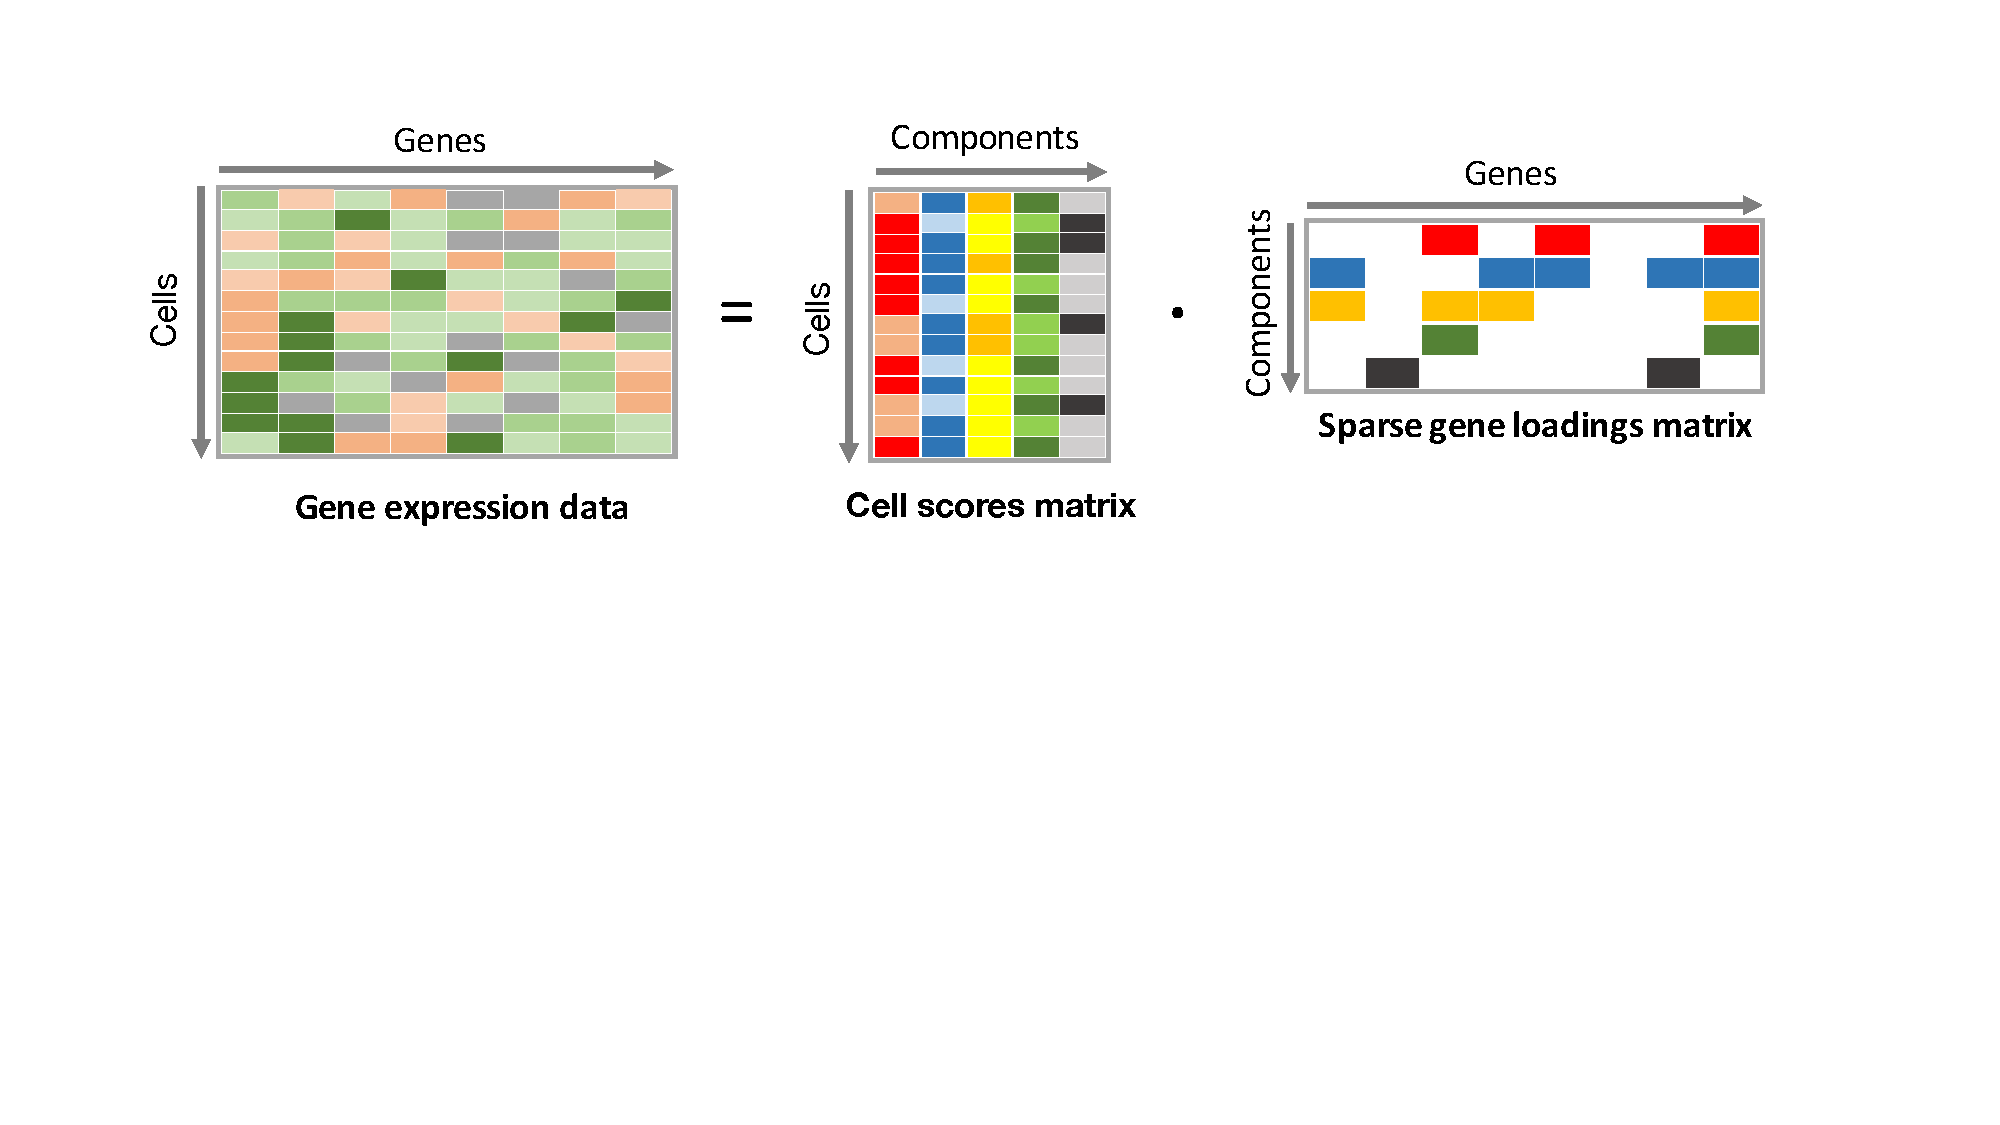
\includegraphics[width=\textwidth]{figures/intro/matrix_decomp_cells.pdf}
	\caption[SDA Matrix Factorisation]{Schematic of the SDA matrix factorisation. From \parencite{Hore2015Latent}}
	\label{fig:SDAfactorisation}
\end{figure}

Sparse decomposition of Arrays (SDA) is a sparse Bayesian factor analysis method, originally developed for decomposing a tensor of multi-tissue bulk RNAseq data, but can also be used in a group factor decomposition mode or to decompose a single 2D matrix (figure \ref{fig:SDAfactorisation}) \parencite{Hore2015Latent, Hore2016Tensor}. The full model for the single matrix decomposition is given in equation \ref{eq:SDA} and in figure \ref{fig:SDAmodel}.

\begin{equation}
\begin{aligned}
y_{n l} &= \sum_{c=1}^{C} a_{n c} x_{c l}+\epsilon_{n l} \\
P(\mathcal{Y} | \theta) &=\prod_{l} \mathcal{N}_{N}\left(\mathbf{y}_{l} | \sum_{c} \mathbf{a}_{\cdot c} x_{c l}, \lambda_{l}^{-1} I_{N}\right) \\ 
P\left(a_{n c}\right) &=\mathcal{N}\left(a_{n c} | 0,1\right) \\
x_{c l} &= w_{c l} s_{c l} \\
P\left(w_{c l} | \beta_{c}\right) &=\mathcal{N}\left(w_{c l} | 0, \beta_{c}^{-1}\right) \\
P\left(\beta_{c}\right) &=\mathcal{G}\left(\beta_{c} | e, f\right) \\ 
P\left(s_{c l} | \psi_{c l}, \phi_{c l}\right) &=\mathcal{B} \text{ernoulli}\left(s_{c l} | p_{c l}\right) \\ 
p_{c l} &= \psi_{c l} \phi_{c l} \\
P\left(\psi_{c l}\right) &=\mathcal{B} \operatorname{eta}\left(\psi_{c l} | g, h\right) \\
P\left(\phi_{c l} | \rho_{c}\right) &=\mathcal{B} \text{ernoulli}\left(\phi_{c l} | \rho_{c}\right) \\
P\left(\rho_{c}\right) &=\mathcal{B} \operatorname{eta}\left(\rho_{c} | r, z\right) \\
P\left(\lambda_{l}\right) &=\mathcal{G}\left(\lambda_{l} | u, v\right) 
\label{eq:SDA}
\end{aligned}
\end{equation}

\begin{figure}[H]
	\centering
	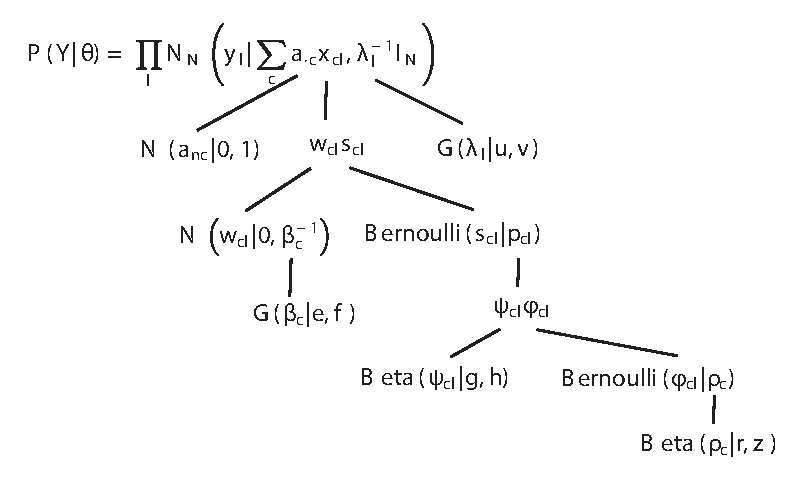
\includegraphics[width=\textwidth]{figures/intro/SDA.pdf}
	\caption[SDA Model]{Schematic of the SDA Hierarchical Bayesian Model}
	\label{fig:SDAmodel}
\end{figure}

$\mathcal{Y}$ is an $N$ by $L$ matrix of cells by genes, $\mathcal{A}$ is a matrix of $N$ cells by $C$ components, and $\mathcal{X}$ is a matrix of $C$ components by $L$ genes, and $\mathcal{E}$ is an $N$ by $L$ matrix of independent Gaussian noise.

A key feature of this model is the element wise sparsity of the gene loadings which eases interpretation of the model, forms a kind of regularisation, and prevents the solution from being rotationally invariant. Moreover this reflects a prior that generally only a subset of genes should be involved in any one biological process. This sparsity is achieved by using a spike and slab prior which is a mixture of a point mass at 0 (spike) and a normal distribution (slab). The slab $w$ has a precision of $\beta_{c}$ which has a Gamma prior with hyper-parameters $e = 10^{-6}$ and $f = 10^{-6}$ (uninformative). The spike $s$ is modelled as a Bernoulli distribution with probability parameter $p_{cl}$ representing the probability of an individual gene loading being non-zero. The prior on this parameter is itself a spike and slab with the slab $\psi_{c l}$ having a Beta prior with hyper-parameters $g=0$ and $h=0$ (a prior with half mass at 0 and half at 1). The spike $\phi_{c l}$ again has a Bernoulli prior with parameter $\rho_{c}$ which also has a Beta prior with hyper-parameters $r=1$ and $z=1$ (flat). This hierarchical structure encourages sparsity as when $\rho_{c}$ is close to 0 the prior on the main spike and slab will be dominated by the spike. The factored spike and slab is equivalent to the pure mixture as in equation \ref{eq:SSMix} but aids inference.

\begin{equation}
P\left(x_{c l} | p_{c l}, \beta_{c}\right)=p_{c l} \mathcal{N}\left(x_{c l} | 0, \beta_{c}^{-1}\right)+\left(1-p_{c l}\right) \delta_{0}\left(x_{c l}\right)
\label{eq:SSMix}
\end{equation}

Each cell score has a standard normal prior. Due to scaling indeterminacy (for example the cell scores could be multiplied by two and gene loadings halved with equivalent fit), the variances are set to 1 with any scaling occurring in the $\beta_{c}$ of the gene loadings. The sign of the components is also unidentifiable, in addition to permutation of the components.

Each gene has a noise precision parameter $\lambda_{l}$ with a Gamma prior where the hyper-parameters are set to $u = 10^{-6}$ and $v = 10^{-6}$ giving an uninformative prior. 

The model is fit using variational Bayes as described in \parencite{Hore2015Latent, Hore2016Tensor}. As variational Bayes underestimates variances the mean of the posterior distributions are used rather than the distributions themselves \parencite{Jaakkola2000Bayesian}. Sparse factor analyses using the spike and slab prior have also previously been used \parencite{West2003Bayesian, Lucas2006Sparse}. The complexity is $\mathcal{O}(NLC^2)$ and the number of components must be chosen ahead of time, although SDA can set entire components to zero if too many components are set.

%\begin{figure}[H]
%	\centering
%	\includegraphics[width=\textwidth]{figures/intro/pseudotime_methods.png}
%	\caption[Pseudotime Methods]{Comparison of pseudotime inference methods, reproduced from~\cite{Cannoodt2016Computational}}
%	\label{fig:pseudotime_methods}
%\end{figure}


% Similar aims (delineating lineage hierarchies and transcriptional networks) have been achieved using single cell RNA-seq in tissues other than testis, highlighting the feasibility of this study~\cite{Trapnell2014Dynamics,Treutlein2014Reconstructing,DurruthyDurruthy2014Reconstruction,Moignard2013Characterization,Stegle2015Computational}.

%\subsection{Principal Components Analysis}

%\subsection{Sparsity}

%Frequentist
%Bayesian
